\section{Auswertung}
\label{sec:Auswertung}

\subsection{statische Methode}
In diesem Kapitel werden die Unterschiede und Gemeinsamkeiten der vier 
Temperaturverläufe $T1$, $T4$, $T5$, $T8$ zu den unterschiedlichen Materialien 
ausgewertet. Weiterhin wird der Stab mit der besten Wärmeleitung bestimmt und 
der Wärmestrom zu jeder Messzeit. Letztlich werden noch die Temperaturdifferenzen 
$\Delta T_{ST}=T7-T8$ und $T_{ST}=T2-T1$ als Funktionen der Messzeit t dargestellt.

\subsubsection{Temperaturverläufe und Wärmeleitung}
\begin{figure}[H]
    \centering
    \includegraphics[width=\textwidth]{tempverlaufT1T4.pdf}
    \caption{Temperaturverläufe von $T1$ und $T4$.}
    \label{fig:f1}
\end{figure}
Bei den beiden Stäben aus \autoref{fig:f1} handelt es sich um Messingstäbe. Der 
Temperaturverlauf verhält sich demnach ziemlich ähnlich. Die Abweichung zwischen 
beiden Verläufen ist mit dem Flächenunterschied zu begründen; die Stäbe von 
T1 und T4 sind unterschiedlicher Größe und da nach \autoref{eqn:1} die Fläche
$A$ proportional zu der Wärmemenge $dQ$ ist, weist T1 eine etwas höhere Temperatur 
auf. Die Abweichung nach oben ist mit einem Messfehler verbunden, welcher noch 
zu diskutieren ist.
\\
In \autoref{fig:f2} befindt sich der Temperaturverlauf des Aluminiumstabs(T5)
und des Edelstahlstabs(T8).
\begin{figure}[H]
    \centering
    \includegraphics[width=\textwidth]{tempverlaufT5T8.pdf}
    \caption{Temperaturverläufe von $T5$ und $T8$.}
    \label{fig:f2}
\end{figure}
\noindent Es ist zunächst zu erkennen, dass der Temperaturverlauf des
Aluminiumstabs recht stark von dem des Edelstahlstabs abweicht. Dieser Verlauf
lässt sich mit der höheren Wärmeleitfähigkeit des Aluminiums erklären. Im 
Vergleich mit den anderen Werten zum Zeitpunkt $t$ = 700s:
\begin{center}
  $T1$ = 43,65°C\\
  $T4$ = 41,41°C\\
  $T5$ = 46,24°C\\
  $T8$ = 33,62°C
\end{center}
Der Aluminiumstab verfügt demnach offenbar über die stärkste Wärmeleitfähigkeit.
Nun lässt sich der Wärmestrom berechnen, indem \autoref{eqn:1} umgeformt wird nach:
\begin{equation}
  \frac{\Delta Q}{\Delta t} = - \kappa A \frac{\partial T}{\partial x}
\end{equation}
Dabei ist $\partial T = T_i - T_j$ und $\partial x$ die ausgemessene Größe von 
0,03m.

In folgender Tabelle wird der Wärmestrom zu 5 unterschiedlichen Zeiten dargestellt.
$\Delta Q_{T1-T2}$ steht für den Wärmestrom zwischen $T1$ und $T2$, analog ergibt 
sich der Wärmestrom $\Delta Q_{T8-T7}$ zwischen den Thermoelementen $T7$ und $T8$.
\begin{table}[H]
  \centering
  \caption{Wärmestrom für 5 Zeiten}
  \label{tab:1}
  %\sisetup{table-format=1.1, per-mode=reciprocal}
  \begin{tblr}{
      colspec = {S S S},
      row{1} = {guard, mode=math},
      %vline{4} = {2}{-}{text=\clap{$\pm$}},
    }
    \toprule
    % t/s & $\Delta Q_{T1-T2}/ \Delta t$ & $\Delta Q_{T8-T7}/ \Delta t$\\
    t/s & \Delta Q_{T1-T2} / \Delta t & \Delta Q_{T8-T7} / \Delta t \\
    \midrule
    100 & 1 & 2 \\
    200 & 1 & 2 \\
    400 & 1 & 2 \\
    600 & 1 & 2 \\
    800 & 1 & 2 \\
    \bottomrule
  \end{tblr}
\end{table}





\subsubsection{Temperaturdifferenz}
In \autoref{fig:f3} ist die Temperaturdifferenz der ersten beiden Thermoelemente 
zu sehen.
\begin{figure}[H]
  \centering
  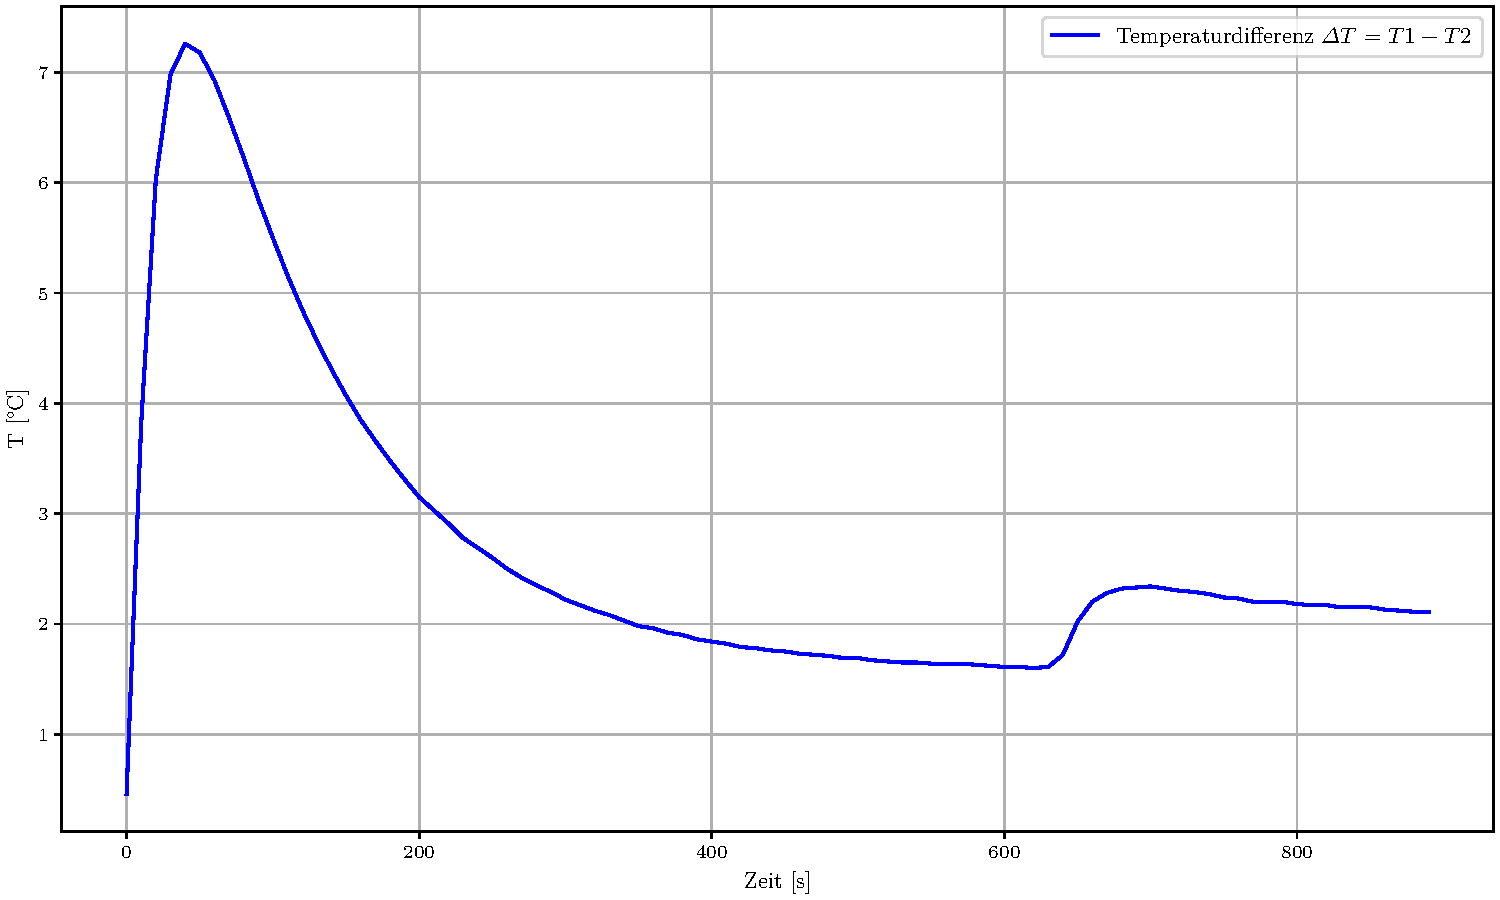
\includegraphics[width=\textwidth]{plotdiff12.pdf}
  \caption{Temperaturdifferenz $T1$ und $T2$.}
  \label{fig:f3}
\end{figure}
In folgender Abbildung befindet sich die Differenz der letzten beiden Thermoelemente.
Dabei fällt auf, dass sich die zeitlichen Entwicklungen ähneln; nach Erreichen 
einer Maximaltemperatur fällt der Graph asymptotisch, wobei der Graph aus 
\autoref{fig:f4} temperaturmäßig weiter oben liegt und nicht so stark sinkt, wie 
der Graph aus \autoref{fig:f3}, was durch die bessere Wärmeleitfähigkeit des Messings 
im Gegensatz zum Edelstahl zu begründen ist. Die erste maximale
Temperaturdifferenz liegt dabei bei etwa 7,3°C und beim Zweiten Graphen bei 
knapp 12,1°C. Auffällig bei beiden Graphen ist wieder der Messfehler am rechten
Ende des Graphen. Dieser wird in der Diskussion behandelt. 
\begin{figure}[H]
  \centering
  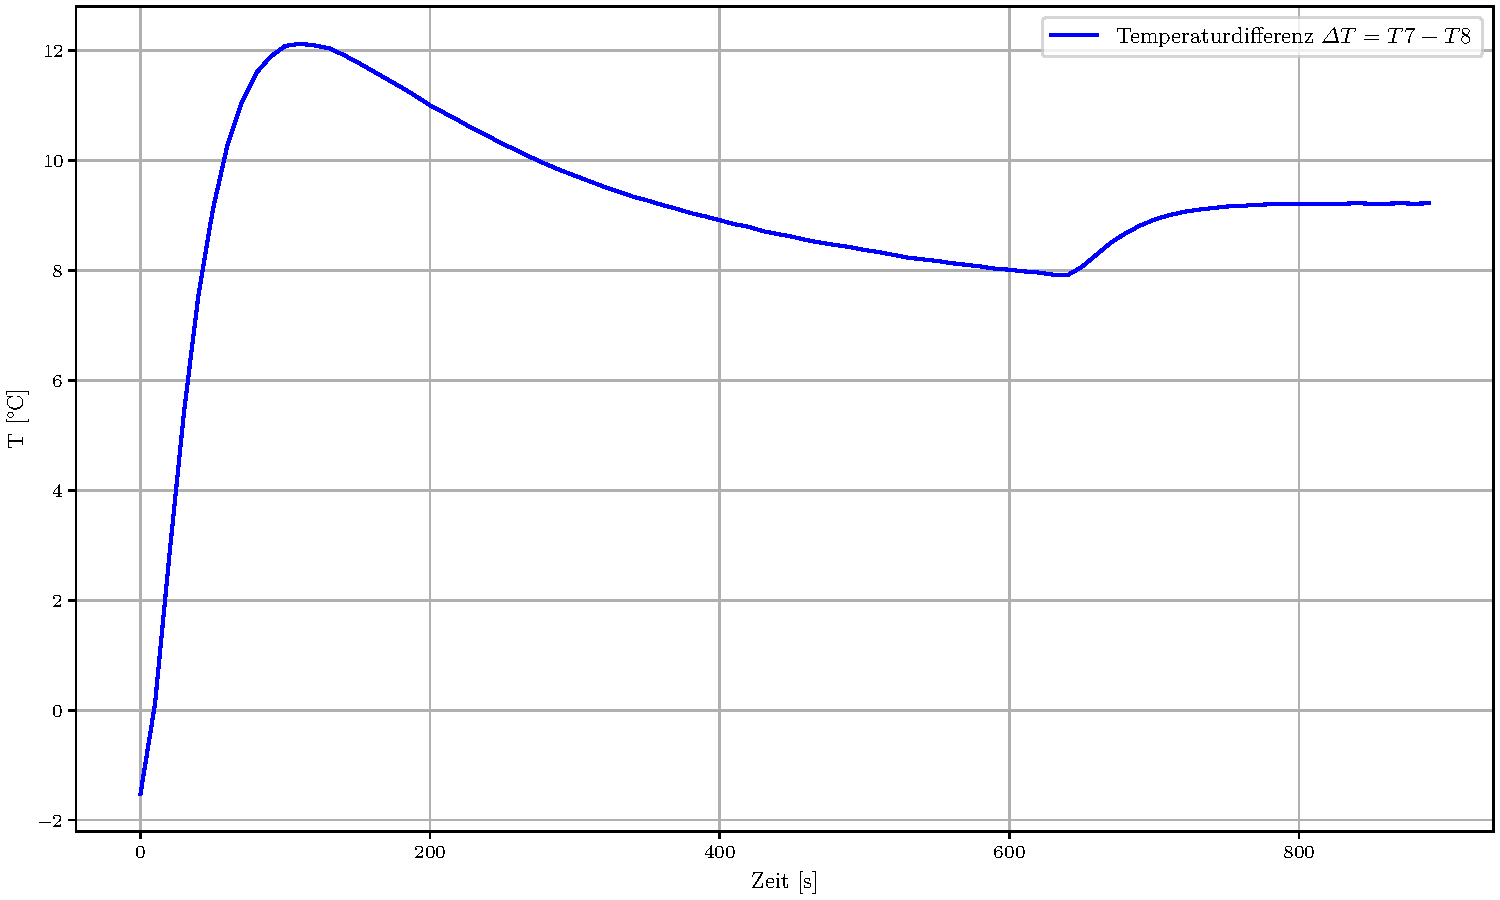
\includegraphics[width=\textwidth]{plotdiff78.pdf}
  \caption{Temperaturdifferenz $T7$ und $T8$.}
  \label{fig:f4}
\end{figure}

\subsection{Dynamische Methode}
Hier wird die Wärmeleitfähigkeit für den Breiten Messingstab, den Aluminiumstab und den Elelstahlstab
mithilfe der in der \autoref{sec:Auswertung} erwähnten Dynamischen methode ermittelt.
\subsubsection{Wärmeleitfähigkeit Messing}
Zur berechnung der Wärmeleitfähigkeit von Messing werden Die messwerte des dicken Messsingstabes
mit den Temperaturmesselementen $T_1$ und $T_2$ benutzt. Jene Wärmeleitfähigkeit lässt sich mit
\autoref{} bestimmen. Darin sind $\Delta x = 0.03/\unit{\meter}$ der Abstand der Temperaturmesselemente, $c$ die Materialabhängige
Wärmekapazität, $\rho $ die Dichte des Stabes, $\Delta t$ die Phasendifferenz
zwischen der Temperaturwelle am Ersten und zweiten Temperaturelement und $A_{nah(fern)}$ 
die Amplitude der Jewailigen Temperaturwellle. Die Ampituden werden durch die 
funktion "find\_peaks" aus der bibiliothek SciPy, angewendet auf die Messdaten, bereitgestellt. 

\begin{table}[H]
  \centering
  \caption{Ermittelte Amplituden und Phasendifferenz}
  \label{tab:2}
  %\sisetup{table-format=1.1, per-mode=reciprocal}
  \begin{tblr}{
      colspec = {S S S S},
      row{1} = {guard, mode=math},
    }
    \toprule
    A_{nah} & A_{fern} & \ln{\frac{A_{nah}}{A_{fern}}} & \Delta t \unit{\second}\\
    \midrule
    1.00  &1.91  &-0.648 &28\\
    0.89  &1.87  &-0.734 &20\\
    0.72  &1.69  &-0.847 &18\\
    0.77  &1.83  &-0.863 &14\\
    0.60  &1.59  &-0.966 &14\\
    0.62  &1.63  &-0.956 &14\\
    0.57  &1.60  &-1.020 &12\\
    0.48  &1.50  &-1.144 &14\\
    0.52  &1.52  &-1.066 &12\\
    0.52  &1.52  &-1.059 &12\\
    \bottomrule
  \end{tblr}
\end{table}
\noindent in \autoref{tab:2} sind die nach \autoref{eqn:} ermittelten Amplituden, sowie der Logarythmus der Amplituden und 
die Phasendifferenz $\Delta t$ aufgeführt. Des weiteren sind in \autoref{abb:mp} die Messwerte, sowie die ermittelten
Hoch und Tiefpunkte Grafisch dargestellt.

\begin{figure}[H]
  \label{abb:mp}
  \centering
  \caption{Graphische Darstellung der gemessenen Temperaturen $T_1$ und $T_2$ pro vergangener Sekunde}
  \includegraphics{messingPlot}
\end{figure}

\noindent Mit den Folgenden Materialeigenschaften $\rho$ und $c$, dem Abstand $\Delta x$, sowie den 
Gemittelten Größen $\Delta t $ und $ \ln{\frac{A_nah}{A_fern}}$ aus den im vorherigen ermittelten Größen, 
lässt sich Das Die Wärmeleitfähigkeit von Messing über \autoref{eqn:} bestimmen. Die Mittelwerte und 
der zugehörige Fehler wurden nach \autoref{} bestimmt.
\begin{align*}
  \rho_M                                &= \qty{8520}{\kilo\gram\per\cubic\meter}\\
  \Delta x                              &= \qty{0.03}{\meter}\\
  c_M                                   &= \qty{385}{\joule\per\kilo\gram\kelvin}\\
  \overline{\ln{\frac{A_nah}{A_fern}}}  &= \qty{-0.93(0.04)}{}\\
  \overline{\Delta t}                   &= \qty{15.45(1.4)}{\second}
\end{align*}

\noindent Die Berechnung der Wärmekapazität Ergibt nach einsetzen der Werte
\begin{equation}
  \kappa_{Messing} = \qty{-103(11)}{\watt\per\meter\kelvin}.
\end{equation}

